\documentclass[12pt]{article}

\usepackage[margin=0.8 in]{geometry}
\usepackage{amsmath}
\usepackage{amssymb}
\usepackage{mathtools}
\usepackage{enumerate}
\usepackage{verbatim}
\usepackage{amsthm}
\usepackage{hyperref}

\title{}
%\content{}



\let \proj \undefined
\newcommand{\p}{\partial}
\newcommand{\R}{ \mathbb{R}}

\DeclareMathOperator{\proj}{proj}
\newcommand{\sS}{\mathscr{S}}
\DeclareMathOperator{\comp}{comp}
\newcommand{\A}{\mathcal{A}}
\newcommand{\D}{\mathcal{D}}
\newcommand{\e}{\epsilon}
\newcommand{\et}{\tilde{\e}}
\newcommand{\vr}{\vec{r}{}}
\newcommand{\vF}{\vec{F}}
\newcommand{\triple}{\iiint_E f(x,y,z)dV}
\renewcommand{\lg}{\langle}
\newcommand{\rg}{\rangle}
\newcommand{\Q}{\frac{\p Q}{\p x}}
\renewcommand{\P}{\frac{\p P}{\p y}}
\let\implies\Rightarrow

\newenvironment{solution}
  {\begin{proof}[Solution]}
  {\end{proof}
  
  }
\newtheorem{example}{Example}
\newtheorem{exercise}{Exercise}
\newtheorem{theorem}{Theorem}
\newtheorem{definition}{Definition}

%
\begin{document}
\section*{The Fundamental Theorem of Calculus for Line Integrals}
What to know:
\begin{enumerate}
\item Be able to state the FTC for conservative vector fields.
\item Know that line integrals of \textbf{conservative} vector fields only depend on initial and terminal point of the path, and are 0 along closed paths.
\item Be able to determine if a set is simply connected by looking at a picture.
\item Be able to check if a vector field defined on a subset of $\R^2$ is conservative.
\item Be able to find a potential function for a conservative vector field and use it to compute line integrals.
\end{enumerate}

Recall from Math 125 that the Fundamental Theorem of Calculus was a tool that related the integral of the derivative of a function over an interval with its values at the endpoints:
\begin{equation}
\int_a^b f'(x)dx=f(b)-f(a)
\end{equation}

Our goal is to generalize this for line integrals of vector fields. Suppose $\vF(x,y)=\nabla f (x,y)$ is a conservative vector field, and a curve $c(t)=\lg x(t),y(t)\rg$, for $t\in [a,b]$. Then, we may write \begin{align*}
\int_c \vF\cdot d\vr=&\int_c\nabla f\cdot d\vr\\
=&\int_a^bf_x (x(t),y(t))x'(t)+f_y(x(t),y(t))y'(t)dt\\
=&\int_a^b\frac{d}{dt}(f(\vr(t))dt\\
=&f(c(b))-f(c(a)),
\end{align*}
using the chain rule and the FTC.

This gives us our theorem:
\begin{theorem} Let $c(t)=\lg x(t),y(t)\rg$, $t\in[a,b]$ be a piecewise smooth curve and $\vF=\nabla f$ a conservative vector field. Then\begin{equation}\int_c \vF\cdot d\vr =f(c(b))-f(c(a)).\label{eq1}\end{equation}
\end{theorem} The same theorem holds for curves in $\R^3$ as well.

\begin{example} Find the work produced by the gravitational force $$\vF(x,y,z)=-\frac{mMG}{(x^2+y^2+z^2)^{3/2}}\lg x,y,z\rg$$ between an object of mass $M$ at the origin and an object of mass $m$ at $(x,y,z)$, while the latter is moving along the path $c(t)=\lg \sin(t),\cos(t),t/2\pi\rg$, $t\in[0,2\pi]$.
\end{example}
\begin{solution}
Recall that the gravitational vector field is conservative and $f(x,y,z)=\dfrac{mMG}{(x^2+y^2+z^2)^{1/2}}$ is a potential function for it. So, by FTC, \begin{align*}\int_c \vF\cdot d\vr =&f(c(b))-f(c(a))\\
=& f(0,1,1)-f(0,1,0)\\
=&\dfrac{mMG}{\sqrt{2}}-\dfrac{mMG}{1}
\end{align*}
\end{solution}


\textbf{Remarks:} Look at the right hand side of \eqref{eq1}: $c$ doesn't appear, only its initial and terminal points. Therefore, \textbf{for conservative vector fields}, the line integral does \textbf{not } depend on the path, only on its initial and terminal point. Stating this more formally, if $\vF$ is conservative and $c_1$, $c_2 $ are two curves so that $c_1(a)=c_2(a)$ and $c_1(b)=c_2(b)$ then $$\int_{c_1}\vF\cdot d\vr =\int_{c_2}\vF\cdot d\vr.$$

In addition, if the path is closed (that is, $c(a)=c(b)$), then the integral of a \textbf{conservative} vector field is 0! This is the justification for calling a vector field conservative: the energy is conserved along closed paths: that is, whatever energy the force gives to an object moving inside a closed path, it takes it back. In the example of the gravitational vector field, think of when you jump: gravity gives you potential energy while you are ascending, but you lose it while descending. In contrast to that, friction is not conservative: it only removes energy from a moving object without ever giving any of it back.


\vspace{.2 in}
Why is the property of being conservative useful? Because if we have a conservative field and want to compute the line integral along a path we can make our lives easier by using one of the following two ideas (mainly the second one):
\begin{enumerate}
\item integrate over a very simple path connecting the endpoints of the path, such as a line segment; it doesn't matter what we choose, we should find the same answer. For instance, in the previous example you could also integrate $\vF$ over the line segment connecting $(0,1,0)$ and $(0,1,1)$.
\item more importantly, find a potential function and use the FTC.
\end{enumerate}

\subsubsection*{How can we tell if a vector field is conservative?}
In your first calculus courses, you might remember that once we had a continuous function $g$, we could always find a function $h$ so that $h'=g$, called an antiderivative, and we did that by integrating, i.e. setting $$h(x)=\int_a^x g(t)dt.$$

Question: Is it possible to do something analogous for two or three dimensions, that is, once we have a continuous or differentiable vector field, can we ``integrate'' it and find a potential function? The answer is \textbf{sometimes}.

Suppose we have a vector field $$\vF(x,y)=\lg P(x,y), Q(x,y)\rg $$ defined on $D\subset \R^2$, where $p$ and $Q$ are continuously differentiable. Then, if we assume that $f (x,y)$ is a potential function, we'd have \begin{align*}
P(x,y)=&f_x(x,y)\\
Q(x,y)=&f_y(x,y)
\end{align*}
Differentiating the first equation with respect to $y$ and the second with respect to $x$, we find $$\P(x,y)=\Q(x,y)\text{ for all }(x,y)\in D,$$ by Clairaut's theorem. So we have the following theorem:

\begin{theorem} If $\vF(x,y)=\lg P(x,y), Q(x,y)\rg$, defined on $D\subset \R^2$, where $p$ and $Q$ are continuously differentiable, is a \textbf{conservative} vector field, then $$\P(x,y)=\Q(x,y)\text{ for all }(x,y)\in D$$
\end{theorem}

\textbf{Remark:} Here it's important that we are doing this in 2 dimensions, it looks different in 3!

So, if we are given a vector field on a domain $D$ and $\P(x,y)\neq \Q(x,y)$ even at one point in $D$, $\vF$ is not conservative! That is, this theorem can tell that a vector field is \textbf{not} conservative, if $\P(x,y)\neq \Q(x,y)$ somewhere, but it doesn't say much about whether it is.

Question: Can we say that the converse is true? That is, if we know that $$\P(x,y)=\Q(x,y)\text{ for all }(x,y)\in D$$ does this tell us that the vector field is conservative? Do the following exercise:

\begin{exercise}
Let $\vF(x,y)=\lg \frac{-y}{x^2+y^2},\frac{x}{x^2+y^2}\rg=\lg P(x,y),Q(x,y)\rg$, defined on $\R^2\backslash \{(0,0)\}$ (the plane without the origin). \begin{enumerate}
\item Compute $\P $ and $\Q$ on $D$.
\item Compute $\int_c \vF\cdot d\vr$, where $c(t)=(\cos(t),\sin(t)),$ $t\in[0,2\pi]$ (the unit circle).
\end{enumerate}
\end{exercise}

If you did the previous exercise, you'd find that the integral over a closed path is not zero. The reason why in this case $\P(x,y)=\Q(x,y)$ on $D$ does \textbf{not} imply that $\vF$ has a potential function is that the domain has a hole in the middle. 

\begin{definition} (A bit informal)
A domain $D\subset \R^2$ that consists of one piece and has no holes is called \textbf{simply connected}.
\end{definition}
\textbf{Remark:} This definition doesn't work in dimensions $\geq 3$: it is a bit more complicated then.

\begin{figure}[h]
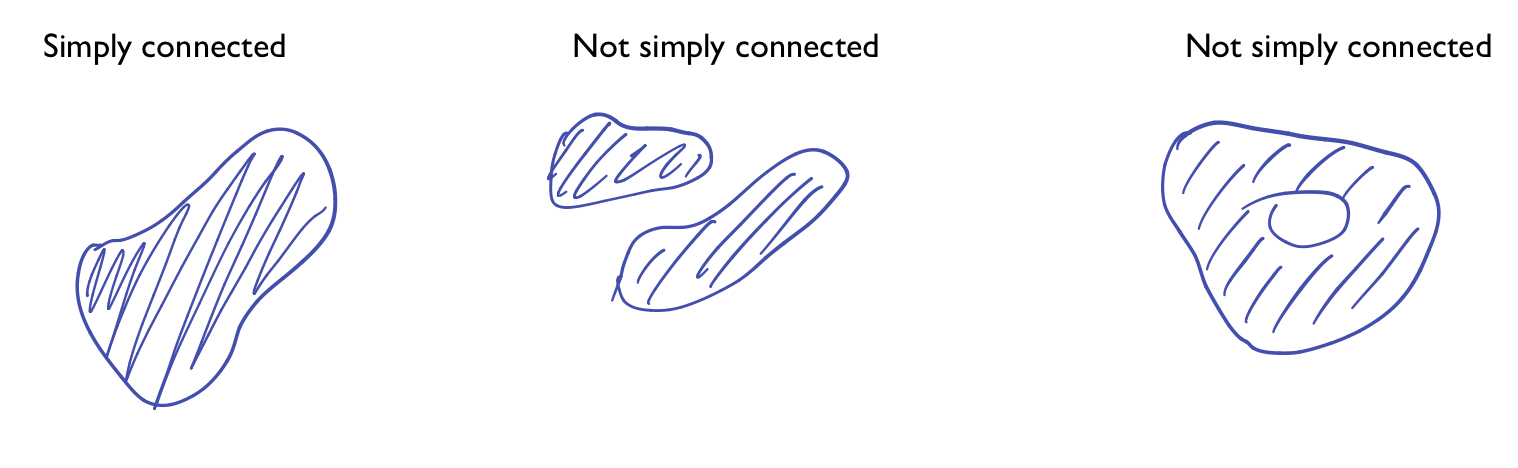
\includegraphics[scale=.3]{sets.jpeg}
\end{figure}

We have the following:
\begin{theorem}  If $\vF(x,y)=\lg P(x,y), Q(x,y)\rg$, defined on a \textbf{simply connected domain} $D\subset \R^2$, where $P$ and $Q$ are continuously differentiable and $$\P(x,y)=\Q(x,y)\text{ for all }(x,y)\in D$$ then there exists a potential function $f$ for $\vF$ on $D$, that is, $\vF=\nabla f$ on $D$.%
\end{theorem}

\textbf{Remark:} Again, this theorem holds as is in 2 dimensions only!

\subsubsection*{How do we find a potential function once we know it exists?}
Once we are given a vector field $\vF(x,y)=\lg P(x,y), Q(x,y)\rg$ in $D\subset \R^2$, here are the steps we take:
\begin{enumerate}
\item Check that $\P(x,y)=\Q(x,y)\text{ for all }(x,y)\in D$ and $D$ is simply connected, to make sure the potential function exists.
\item Integrate $P$ with respect to $x$ to find $f(x,y)=\int P(x,y)dx +g(y)$.
\item Differentiate the result with respect to $y$, set $\frac{\p f}{\p y }=Q$.
\item Integrate with respect to $y$ to determine $g$.
\end{enumerate}

Let's see how this works in an example:
\begin{example}
Let $\vF(x,y)=\lg 2xy, x^2+6y^2\rg$ on $\R^2$. Determine if $\vF$ is conservative and find a potential function, if it is.
\end{example}
\begin{solution}
We set $\vF(x,y)=\lg P(x,y), Q(x,y)\rg$ and find that \begin{align*}
\P&=\frac{\p}{\p y}(2xy)=2x\\
\Q&=\frac{\p}{\p x}(x^2+6y^2)=2x
\end{align*}
so, since $\R^2 $ is simply connected, $\vF$ is conservative. Let's find a potential function, call it $f$. We need $\vF = \nabla f$, so \begin{align}
f_x=2xy\label{eq2}
\end{align} and \begin{align}
f_y=x^2+6y^2.\label{eq3}
\end{align}
Then integrating the first one with respect to $x$, we find $$f(x,y)=x^2y+\phi(y).$$
This is saying that the constant of integration with respect to $x$ doesn't have a reason to not depend on $y$! Therefore, we have to think of it as a function of $y$.

To make use of \eqref{eq3}, we differentiate  with respect to $y$:
\begin{align}
f_y=x^2+\phi '(y).
\end{align}
So, using  \eqref{eq3}, $$x^2+\phi '(y)=x^2+6y^2$$ and we may finally integrate with respect to $y$ and find $$\phi(y)=2y^3+c,$$ and therefore $$f(x,y)=x^2y+2y^3+c.$$
\end{solution}

\subsubsection*{Finding potential functions in $\R^3$}
The above discussion doesn't give information about determining whether a vector field in $\R^3$ is conservative. We will see such a criterion in the sections to come.

Here's how we find a potential function for a vector field on a subset of $\R^3$ once it is given that it is conservative.
\begin{example}
It is known that $\vF(x,y,z)=\lg 2x, 6zy^2, 2y^3+2\rg $ is conservative. Find a potential function $f$ for it.
\end{example}
\begin{solution}Set
\begin{align}
P(x,y,z)=&2x\\
Q(x,y,z)=&6zy^2\\
R(x,y,z)=&2y^3+2.
\end{align}
Then $f_x=P\implies f_x=2x\implies f(x,y,z)=x^2+g(y,z)$, for some $g(y,z)$. Then $f_x=g_y$, so $$g_y=Q=6zy^2.$$

This gives $$g(y,z)=2zy^3+h(z).$$ So $$f(x,y,z)=x^2+2zy^3+h(z)\implies f_z=2y^3+h'(z).$$

Finally, $f_z=R=2y^3+2$ means $h'(z)=2\implies h(z)=2z+c$. Therefore, $$f(x,y,z)=x^2+2zy^3+2z+c.$$
\end{solution}


\subsubsection*{An optional remark about Exercise 1}
In Exercise 1, you should have found that $\P=\Q$ on $D=\R^2\backslash \{(0,0)\}$. As we saw, we can't find a potential function for $\vF$ on $D$, since this would have to imply that the line integral over the unit circle is 0. However, we could still restrict our interest in any simply connected subset of $\R^2\backslash \{(0,0)\}$ and find a potential function there (for example, you could take a disk of radius 1 centered at (2,0)). 

You can follow the procdure described before for computing potential functions, and find that in any such domain a potential function for $\vF$ is $f(x,y)=\arctan(\frac{y}{x})$, which looks more familiar in polar coordinates: $f(\rho,\theta)=\theta$!. This function can be defined to be differentiable in any simply connected subset of $D$, but not everywhere on $D$: after completing a full rotation, the angle $\theta$ has jumped by $2\pi$ and therefore can't be continuous!.







\end{document}

